% !TeX program = xelatex
% 用户上传原书的非官方译注稿，原书翻译和公开传播权归权利人。
\documentclass[lang=cn,color=blue,11pt]{elegantbook}
\usepackage{amsmath,amssymb,mathtools,bm}
\usepackage{tikz}
\usetikzlibrary{arrows.meta,calc}
\newcommand{\exproblem}[2]{\par\bigskip\noindent\textbf{\large 原书第\,#1\,题}\hfill{\small 原书印刷页 #2}\par\smallskip}
\newcommand{\exsolution}{\par\medskip\noindent\textbf{【详细解析】}\quad}
\newcommand{\excheck}{\par\smallskip\noindent\textbf{【核验】}\quad}
\title{《普通物理学习题》中文译注与详解}
\subtitle{Problems in General Physics --- 逐题整理（进行中）}
\author{原著：I. E. Irodov \quad 中文译注与题解：三千弱水}
\date{2026年11月21日 · 第一批：1--20题}
\version{0.1}
\cover{cover.pdf}
\begin{document}
\maketitle
\frontmatter
\chapter*{编辑说明}
以用户上传的 Arihant 版 \emph{Problems in General Physics}（PDF共385页）为底本。
本批仅包括第一篇第一章第一节“运动学”第1--20题，\textbf{全书尚未译完}。
原书答案部分以简答为主，本稿补写公式推导、必要条件及核验。第4、17、18题的图以TikZ重绘。
其中第4题示意图不是原曲线的数字化精密拟合，结果依原图读数。
公式已自查，\textbf{不宣称经过独立专家审查}。
\paragraph{记号}
原书以 $\bm w$ 表示加速度，本稿统一记为 $\bm a$。
平均速率为总路程除以总时间；平均速度矢量为总位移除以总时间。
\tableofcontents
\mainmatter
\chapter{力学的物理基础}
\section{运动学：第1--20题}
\exproblem{1}{1}
一艘汽艇顺流行驶，在 $A$ 点赶上随水漂流的木筏。经过 $\tau=60\,\mathrm{min}$ 后汽艇掉头，在距 $A$ 点 $\ell=6.0\,\mathrm{km}$ 处再次与木筏相遇。设汽艇相对水的航速大小不变，求河流速度。

\exsolution
设水流速度为 $u$，汽艇相对水速为 $v$。改在随木筏一起漂移的参考系中观察，木筏静止，汽艇先以 $v$ 行驶 $\tau$，再以相同的速率返航，因此返航时间同样为 $\tau$。木筏在地面系中漂移距离 $\ell=u(2\tau)$，即
\[
\boxed{u=\frac{\ell}{2\tau}=\frac{6.0\,\mathrm{km}}{2.0\,\mathrm h}=3.0\,\mathrm{km/h}.}
\]

\excheck
结果与汽艇相对水的速率无关，只要求顺、逆行驶时该速率的大小相同。


\exproblem{2}{1--2}
质点以速率 $v_0$ 走过全程的一半；余下的半程中，前一半\emph{时间}以速率 $v_1$、后一半时间以速率 $v_2$ 运动。求全程平均速率。

\exsolution
记总路程为 $S$。前半程历时 $t_0=S/(2v_0)$。余下半程历时 $t_1$，有
\[
\frac S2=\frac{v_1t_1}2+\frac{v_2t_1}2
\quad\Longrightarrow\quad t_1=\frac{S}{v_1+v_2}.
\]
所以平均速率
\[
\boxed{\bar v=\frac{S}{t_0+t_1}
=\frac{2v_0(v_1+v_2)}{2v_0+v_1+v_2}.}
\]

\excheck
若 $v_0=v_1=v_2$，则 $\bar v=v_0$；不要混淆相等时间与相等路程。


\exproblem{3}{2}
汽车从静止开始以 $a=5.0\,\mathrm{m/s^2}$ 匀加速，随后匀速，最后以同样大小的减速度停车。总时间 $T=25\,\mathrm s$，全程平均速率 $72\,\mathrm{km/h}$。求匀速时间。

\exsolution
加速段和减速段的历时均设为 $t$，最大速度为 $at$，匀速段历时 $T-2t$。由速度—时间图像的面积求得位移
\[
S=\tfrac12at^2+at(T-2t)+\tfrac12at^2=at(T-t).
\]
又平均速率为 $20\,\mathrm{m/s}$，故
\[
5t(25-t)=20\times25,\quad(t-5)(t-20)=0.
\]
由于匀速时间非负，有 $t\le12.5\,\mathrm s$，故取 $t=5\,\mathrm s$，
\[
\boxed{T_{\rm uniform}=25-2t=15\,\mathrm s.}
\]

\excheck
最大速率 $25\,\mathrm{m/s}$，总位移 $500\,\mathrm m$，和题给平均速率相符。


\exproblem{4}{2}
质点沿直线单向运动。原书图1.1给出路程—时间曲线，求：（a）全程平均速率；（b）最大瞬时速率；（c）使瞬时速率等于从出发至该时刻平均速率的时刻 $t_0$。
\begin{center}
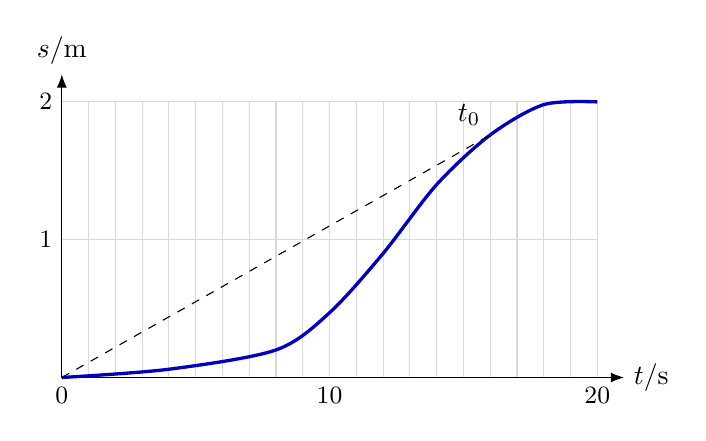
\begin{tikzpicture}[x=.34cm,y=1.75cm,>=Latex]
\draw[gray!30,step=1] (0,0) grid (20,2);
\draw[->] (0,0)--(21,0) node[right] {$t/\mathrm s$};
\draw[->] (0,0)--(0,2.2) node[above] {$s/\mathrm m$};
\foreach \t in {0,10,20}{\node[below] at (\t,0) {\small\t};}
\foreach \s in {1,2}{\node[left] at (0,\s) {\small\s};}
\draw[very thick,blue!75!black] plot[smooth] coordinates {(0,0)(4,.06)(8,.20)(10,.47)(12,.90)(14,1.40)(16,1.76)(18,1.98)(20,2)};
\draw[dashed] (0,0)--(16,1.76);
\node[above left] at (16,1.76) {$t_0$};
\end{tikzpicture}
\end{center}
以上为根据原图重绘的近似示意，并非原图的精密数字化。

\exsolution
（a）平均速率是两端点连线斜率：
\[
\boxed{\bar v=\frac{2.0\,\mathrm m}{20\,\mathrm s}
=10\,\mathrm{cm/s}.}
\]
（b）瞬时速率是曲线在相应时刻的切线斜率。图中最陡切线斜率约为 $0.25\,\mathrm{m/s}$，所以
\[\boxed{v_{\max}\approx25\,\mathrm{cm/s}.}\]
（c）条件 $v(t_0)=s(t_0)/t_0$ 表示从原点引向曲线的一条切线。按原书图读得
\[\boxed{t_0\approx16\,\mathrm s.}\]

\excheck
后两项为图像估读值；精确拟合应使用原图，而不是本稿示意曲线。


\exproblem{5}{2}
两粒子分别以恒速度矢量 $\bm v_1,\bm v_2$ 运动，初始位矢为 $\bm r_1,\bm r_2$。这些矢量满足什么关系时二者相撞？

\exsolution
若在 $t\ge0$ 相撞，则
\[
\bm r_1+\bm v_1t=\bm r_2+\bm v_2t,
\quad \bm r_1-\bm r_2=(\bm v_2-\bm v_1)t.
\]
当初始不同点且相对速度非零时，必要且充分条件是 $\bm r_1-\bm r_2$ 与 $\bm v_2-\bm v_1$ 同向共线；此时
\[
\boxed{t_{\rm col}=\frac{(\bm r_1-\bm r_2)\cdot(\bm v_2-\bm v_1)}
{\lVert\bm v_2-\bm v_1\rVert^2}>0.}
\]
求出的 $t$ 还须满足上面的矢量方程，单独检验点积正值不够。

\excheck
若初始已重合则 $t=0$ 已相撞；若初始不同点、两速度相同，则永不相撞。


\exproblem{6}{2}
一艘船沿赤道向东航行，速度 $v_0=30\,\mathrm{km/h}$。来自东南方向的风速为 $v=15\,\mathrm{km/h}$，与赤道夹角 $\varphi=60^\circ$。求相对船的风速大小与风向角。

\exsolution
以东、北为 $x,y$ 正方向。东南风吹向西北，所以风的地面速度与船速分别为
\[
\bm v_w=(-v\cos\varphi,v\sin\varphi),\qquad \bm v_s=(v_0,0).
\]
相对风速 $\bm v'=\bm v_w-\bm v_s$，故
\[
\boxed{v'=\sqrt{v_0^2+v^2+2v_0v\cos\varphi}
\approx39.7\,\mathrm{km/h}},
\]
\[
\boxed{\varphi'=\arctan\frac{v\sin\varphi}{v_0+v\cos\varphi}
\approx19.1^\circ}.
\]
相对船的风吹向西偏北约 $19^\circ$。

\excheck
向东行驶的船使相对风的向西分量增大，所以夹角小于原来的 $60^\circ$。


\exproblem{7}{2}
两人从河岸 $A$ 游向正对岸 $B$。甲沿直线 $AB$ 游至终点；乙相对水垂直河流游泳后沿岸步行回 $B$。水速 $v_0=2.0\,\mathrm{km/h}$，二人相对水速 $v'=2.5\,\mathrm{km/h}$。若同时到达，求乙的步速 $u$。

\exsolution
记河宽为 $d$。甲向上游的速度分量必须抵消河流，于是垂直河岸的有效速度为 $\sqrt{v'^2-v_0^2}$，渡河时间
\[
t_A=\frac d{\sqrt{v'^2-v_0^2}}.
\]
乙渡河历时 $d/v'$，顺流漂移 $v_0d/v'$，步行历时 $v_0d/(v'u)$，所以
\[
t_B=\frac d{v'}+\frac{v_0d}{v'u}.
\]
由 $t_A=t_B$，解得
\[
\boxed{u=\frac{v_0}{v'/\sqrt{v'^2-v_0^2}-1}
=\frac{2}{2.5/1.5-1}=3.0\,\mathrm{km/h}.}
\]

\excheck
甲可直线横渡需要 $v'>v_0$；未知河宽 $d$ 被消去。


\exproblem{8}{2--3}
两船从河中浮标分别沿顺流方向和垂直水流方向驶出，均到达距离浮标 $L$ 处后按原路返回。每船相对水的速率是河流速率的 $\eta=1.2$ 倍。求两船往返时间比 $T_A/T_B$。

\exsolution
记船相对水速为 $v$，河速为 $u$。顺河方向往返所需时间
\[
T_A=\frac{L}{v+u}+\frac{L}{v-u}=\frac{2Lv}{v^2-u^2}.
\]
横河方向需以大小 $u$ 的上游分量抵消水流，故有效横向速度是 $\sqrt{v^2-u^2}$，时间
\[
T_B=\frac{2L}{\sqrt{v^2-u^2}}.
\]
相除得
\[
\boxed{\frac{T_A}{T_B}=\frac{v}{\sqrt{v^2-u^2}}
=\frac{\eta}{\sqrt{\eta^2-1}}\approx1.81.}
\]

\excheck
$\eta>1$ 是横河运动可按岸上直线往返的必要条件。


\exproblem{9}{3}
船相对水速比河流速率小 $n=2.0$ 倍。为了使横渡时的顺流漂移最小，相对水的行驶方向应与水流成何角度 $\theta$？

\exsolution
设河宽 $d$、水速 $u$、船相对水速 $v=u/n$，与顺流方向夹角 $0<\theta<\pi$。渡河时间与顺流漂移为
\[
T=\frac d{v\sin\theta},\qquad
\Delta x=(u+v\cos\theta)T
=d\frac{n+\cos\theta}{\sin\theta}.
\]
求导：
\[
\frac{\mathrm d}{\mathrm d\theta}
\frac{n+\cos\theta}{\sin\theta}
=-\frac{1+n\cos\theta}{\sin^2\theta}.
\]
驻点满足 $\cos\theta=-1/n$，且漂移在两侧端点趋于正无穷，故驻点为最小值：
\[
\boxed{\theta=\arccos(-1/n)=120^\circ.}
\]

\excheck
因船速小于水速，不能完全消除顺流漂移，只能使其最小。


\exproblem{10}{3}
同一点同时将两物体分别竖直向上和与水平成 $\theta=60^\circ$ 抛出，初速大小同为 $v_0=25\,\mathrm{m/s}$。忽略空气阻力，求 $t=1.70\,\mathrm s$ 后的间距。

\exsolution
以水平、竖直为坐标轴，两物体的位置分别为
\[
\bm r_1=(0,v_0t-\tfrac12gt^2),\quad
\bm r_2=(v_0t\cos\theta,v_0t\sin\theta-\tfrac12gt^2).
\]
相对位移
\[
\bm r_2-\bm r_1=v_0t(\cos\theta,\sin\theta-1).
\]
取模，并利用 $\cos^2\theta+(1-\sin\theta)^2=2(1-\sin\theta)$：
\[
\boxed{D=v_0t\sqrt{2(1-\sin\theta)}
\approx22.0\,\mathrm m.}
\]

\excheck
两物体重力加速度相等，相对加速度为零；最后结果不依赖 $g$。


\exproblem{11}{3}
两质点同地同刻出发，以 $v_1=3.0\,\mathrm{m/s}$ 和 $v_2=4.0\,\mathrm{m/s}$ 的水平初速度反向运动，仅受重力。求两速度矢量互相垂直时的间距。

\exsolution
两速度可写作
\[
\bm v_1(t)=(v_1,-gt),\quad \bm v_2(t)=(-v_2,-gt).
\]
点积为零等价于 $-v_1v_2+g^2t^2=0$，所以
\[
t=\frac{\sqrt{v_1v_2}}g.
\]
二者竖直位移相同，间距就是水平距离，故
\[
\boxed{D=(v_1+v_2)t
=\frac{(v_1+v_2)\sqrt{v_1v_2}}g
\approx2.47\,\mathrm m\simeq2.5\,\mathrm m.}
\]

\excheck
点积条件具有明确的正时刻解；结果量纲为长度。


\exproblem{12}{3}
三个点位于边长为 $a$ 的等边三角形各顶点，并以速率 $v$ 同时运动；第一个始终指向第二个，第二个指向第三个，第三个指向第一个。问何时汇合？

\exsolution
系统始终保持三重旋转对称，故三点组成边长为 $a(t)$ 的等边三角形。设从 $A$ 指向 $B$ 的边方向为 $\bm e$，$A$ 的速度沿 $\bm e$，$B$ 指向第三个点的速度与 $\bm e$ 成 $120^\circ$。边长变化率
\[
\dot a=(\bm v_B-\bm v_A)\cdot\bm e
=v\cos120^\circ-v=-\tfrac32v.
\]
积分至 $a(T)=0$，得到
\[
\boxed{T=\frac{2a}{3v}.}
\]

\excheck
即使每个点沿曲线追逐，三角形边长的缩减速率依然恒定。


\exproblem{13}{3}
质点 $A$ 以恒速率 $v$ 运动，速度始终指向质点 $B$；$B$ 沿直线以恒速率 $u<v$ 运动。初始时 $A$ 的速度垂直于 $B$ 的速度，二者相距 $\ell$。求追及时间。

\exsolution
取 $B$ 的运动方向为 $x$ 轴。设追逐连线与该轴夹角为 $\alpha(t)$，两点距离为 $r(t)$。相对运动在连线上的投影给出
\[
\dot r=u\cos\alpha-v.
\]
到追及时刻 $T$，由 $r(0)=\ell$、$r(T)=0$，
\[
\ell=vT-u\int_0^T\cos\alpha\,\mathrm dt.
\]
初始连线与 $B$ 的运动方向垂直，因此两点相遇时 $A$ 的水平位移等于 $B$ 的 $uT$：
\[
v\int_0^T\cos\alpha\,\mathrm dt=uT.
\]
代回前式整理得
\[
\boxed{T=\frac{v\ell}{v^2-u^2}.}
\]

\excheck
$u\to0$ 时退化为 $\ell/v$；$u\to v^-$ 时追及时间趋于无穷。


\exproblem{14}{3}
列车长 $\ell=350\,\mathrm m$，从静止开始以 $a=3.0\times10^{-2}\,\mathrm{m/s^2}$ 匀加速。$t_1=30\,\mathrm s$ 时车头灯点亮（事件1），再过 $\tau=60\,\mathrm s$ 后车尾灯点亮（事件2）。求两事件在列车附着系和地面系中的空间间隔；求使它们在同一坐标位置发生的匀速参考系速度。

\exsolution
以初始车尾为原点、列车前进方向为正，车头与车尾的地面坐标为
\[
x_H(t)=\ell+\tfrac12at^2,\quad x_T(t)=\tfrac12at^2.
\]
列车附着坐标中事件1在车头、事件2在车尾，故空间间距为 $\boxed{350\,\mathrm m}$。
地面系中 $t_2=t_1+\tau=90\,\mathrm s$，
\[
x_1-x_2=\ell+\tfrac12a(t_1^2-t_2^2)
=\ell-a\tau(t_1+\tau/2)
=350-108=\boxed{242\,\mathrm m}.
\]
若新惯性系以速度 $V$ 匀速运动，则 $x'=x-Vt$。令 $x_1'=x_2'$ 得
\[
\boxed{V=\frac{x_2-x_1}{\tau}=-\frac{242}{60}
\approx-4.03\,\mathrm{m/s}.}
\]

\excheck
负号表示与列车前进方向相反；车厢附着系是加速系而非惯性系。


\exproblem{15}{3}
电梯从静止开始以 $a=1.2\,\mathrm{m/s^2}$ 向上匀加速，轿厢高 $h=2.7\,\mathrm m$。$2.0\,\mathrm s$ 后天花板一颗螺栓掉落。求：（a）落至地板的时间；（b）在电梯井参考系内螺栓的位移和路程。

\exsolution
脱落瞬间螺栓具有向上的地面速度 $v_0=at_0=2.4\,\mathrm{m/s}$。相对电梯的加速度向下、大小为 $g+a$，于是
\[
h=\tfrac12(g+a)T^2,\quad
\boxed{T=\sqrt{\frac{2h}{g+a}}\approx0.701\,\mathrm s}.
\]
以竖直向上为正，螺栓地面位移
\[
\Delta y=v_0T-\tfrac12gT^2\approx-0.725\,\mathrm m.
\]
脱落后它先上升，在 $t_*=v_0/g\approx0.245\,\mathrm s$ 时转而下落；最高点相对脱落位置上升
\[
d_\uparrow=\frac{v_0^2}{2g}\approx0.294\,\mathrm m.
\]
因此总路程为上升加下降长度：
\[
\boxed{s=2d_\uparrow+|\Delta y|
=\frac{v_0^2}{g}+|\Delta y|\approx1.31\,\mathrm m.}
\]

\excheck
位移约为 $0.73\,\mathrm m$ 向下，路程约 $1.31\,\mathrm m$；二者不能混淆。


\exproblem{16}{3--4}
两质点分别以速率 $v_1,v_2$ 沿两条互相垂直的直线朝交点 $O$ 运动，起初距离 $O$ 分别为 $\ell_1,\ell_2$。求两质点间距达到最小的时刻与最小值。

\exsolution
取两路径为两坐标轴。二者位置为
\[
\bm r_1=(\ell_1-v_1t,0),\quad \bm r_2=(0,\ell_2-v_2t).
\]
间距平方
\[
D^2=(\ell_1-v_1t)^2+(\ell_2-v_2t)^2
\]
是严格凸的二次函数。令 $\mathrm d(D^2)/\mathrm dt=0$，有
\[
\boxed{t_*=\frac{\ell_1v_1+\ell_2v_2}{v_1^2+v_2^2}.}
\]
代回并整理平方，得到
\[
\boxed{D_{\min}=\frac{|\ell_1v_2-\ell_2v_1|}
{\sqrt{v_1^2+v_2^2}}.}
\]

\excheck
若 $\ell_1/v_1=\ell_2/v_2$，两质点同时到达 $O$，最短距离为零。


\exproblem{17}{4}
由公路上点 $A$ 开车前往野外点 $B$，$D$ 为 $B$ 到公路的垂足，$BD=\ell$。汽车野外速度是公路速度的 $1/\eta$（$\eta>1$）。应在距 $D$ 多远的 $C$ 点离开公路，才能最快到达？
\begin{center}
\begin{tikzpicture}[scale=.85]
\draw[thick] (0,2)--(7.4,2);
\draw[dashed] (4.7,2)--(6.5,.1);
\draw[thick] (6.5,2)--(6.5,.1);
\node[above] at (.6,2) {$A$};\node[above] at (4.7,2) {$C$};
\node[above] at (6.5,2) {$D$};\node[below] at (6.5,.1) {$B$};
\node[right] at (6.5,1) {$\ell$};
\end{tikzpicture}
\end{center}

\exsolution
设公路速度为 $v$，$AD=L$，$CD=d\in[0,L]$。公路段距离 $L-d$，野外段距离 $\sqrt{d^2+\ell^2}$，总时间
\[
T(d)=\frac{L-d}{v}+\frac{\eta\sqrt{d^2+\ell^2}}{v}.
\]
有
\[
T'(d)=\frac1v\left(-1+\frac{\eta d}{\sqrt{d^2+\ell^2}}\right),\quad
T''(d)=\frac{\eta\ell^2}{v(d^2+\ell^2)^{3/2}}>0.
\]
唯一无约束极小点满足 $\eta d=\sqrt{d^2+\ell^2}$，故
\[
\boxed{CD=\frac{\ell}{\sqrt{\eta^2-1}}.}
\]

\excheck
若 $AD$ 小于上述距离，必须尊重 $d\le AD$，最优解改为从 $A$ 直接驶入野外。


\exproblem{18}{4}
一质点沿 $x$ 轴运动，原书图1.3给出的速度折线经过 $(0,0),(1,1),(3,1),(6,-2),(7,0)$。设 $x(0)=0$，绘出加速度 $a_x$、坐标 $x$ 与路程 $s$ 的时间图像。
\begin{center}
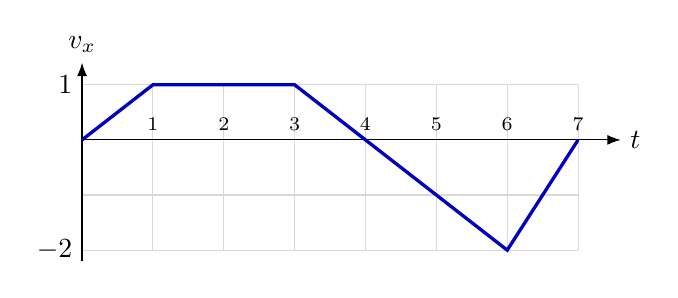
\begin{tikzpicture}[x=.9cm,y=.7cm,>=Latex]
\draw[gray!30,step=1] (0,-2) grid (7,1);
\draw[->] (0,0)--(7.6,0) node[right] {$t$};
\draw[->] (0,-2.2)--(0,1.4) node[above] {$v_x$};
\draw[very thick,blue!75!black] (0,0)--(1,1)--(3,1)--(6,-2)--(7,0);
\foreach \t in {1,2,3,4,5,6,7}{\node[above] at (\t,0) {\scriptsize\t};}
\node[left] at (0,1) {$1$};\node[left] at (0,-2) {$-2$};
\end{tikzpicture}
\end{center}

\exsolution
按折线各段的斜率，先将速度写成
\[
v_x(t)=\begin{cases}
t,&0\le t\le1,\\1,&1<t\le3,\\
4-t,&3<t\le6,\\2t-14,&6<t\le7.
\end{cases}
\]
于是加速度图由四段水平线组成，
\[
\boxed{a_x(t)=\begin{cases}
1,&0<t<1,\\0,&1<t<3,\\-1,&3<t<6,\\2,&6<t<7.
\end{cases}}
\]
在折线的连接点通常不存在普通导数。根据 $x(0)=0$，分段积分且保持连续，得
\[
\boxed{x(t)=\begin{cases}
t^2/2,&0\le t\le1,\\t-1/2,&1<t\le3,\\
5/2+(t-3)-(t-3)^2/2,&3<t\le6,\\
1-2(t-6)+(t-6)^2,&6<t\le7.
\end{cases}}
\]
由于路程是 $\int_0^t|v_x|\,\mathrm dt$，在 $t=4$ 后速度变负，须改变积分符号：
\[
\boxed{s(t)=\begin{cases}
t^2/2,&0\le t\le1,\\t-1/2,&1<t\le3,\\
5/2+(t-3)-(t-3)^2/2,&3<t\le4,\\
3+(t-4)^2/2,&4<t\le6,\\
5+2(t-6)-(t-6)^2,&6<t\le7.
\end{cases}}
\]

\excheck
$x(4)=3$ 为最大坐标，$x(7)=0$；而 $s(4)=3,s(6)=5,s(7)=6$，路程始终不减。


\exproblem{19}{4}
质点在 $T=10.0\,\mathrm s$ 内沿半径 $R=160\,\mathrm{cm}$ 的半圆弧运动。求：（a）平均速率；（b）平均速度矢量模；（c）若切向加速度恒定，平均加速度矢量的模。

\exsolution
半圆弧长 $\pi R$，故平均速率
\[
\boxed{\bar v=\frac{\pi R}{T}\approx50.3\,\mathrm{cm/s}.}
\]
首末位置间位移为直径 $2R$，平均速度矢量的模为
\[
\boxed{\lVert\langle\bm v\rangle\rVert=\frac{2R}{T}=32\,\mathrm{cm/s}.}
\]
切向加速度恒定时，初、末速率 $v_i,v_f$ 满足 $(v_i+v_f)/2=\pi R/T$。由于起终点切线方向相反，速度矢量增量的模为 $v_i+v_f$，故
\[
\boxed{\lVert\langle\bm a\rangle\rVert
=\frac{v_i+v_f}{T}
=\frac{2\pi R}{T^2}\approx10.1\,\mathrm{cm/s^2}.}
\]

\excheck
平均加速度由总速度矢量增量计算，不等于加速度大小的时间平均。


\exproblem{20}{4}
位矢为 $\bm r(t)=\bm b\,t(1-\alpha t)$，$\bm b$ 是恒矢量，$\alpha>0$。求：（a）速度和加速度；（b）返回初始位置所需时间及其间总路程。原书把 $\bm b$ 记为 $\bm a$；为避免与加速度混淆而改用此记法。

\exsolution
微分得
\[
\boxed{\bm v(t)=\bm b(1-2\alpha t),\qquad
\bm a(t)=-2\alpha\bm b.}
\]
初始位置是 $\bm r(0)=\bm0$。求 $t>0$ 满足 $\bm r(t)=\bm0$，得
\[
\boxed{T=\frac1\alpha.}
\]
在 $t_*=1/(2\alpha)$ 速度反向，质点先远离原点后沿同一路径折返。到最远点的距离为
\[
\lVert\bm r(t_*)\rVert
=\left\lVert\bm b\frac1{2\alpha}
\left(1-\frac12\right)\right\rVert
=\frac{\lVert\bm b\rVert}{4\alpha}.
\]
故往返的总路程是此值的两倍：
\[
\boxed{s=\frac{\lVert\bm b\rVert}{2\alpha}.}
\]

\excheck
$\bm b$ 量纲为长度/时间，$\alpha$ 量纲为时间的倒数；总位移为零不代表总路程为零。


\backmatter
\chapter*{版本信息}
本批中文题面及解析为20/20；第4题含近似读图值，第5题补退化条件，第17题补边界条件。
编译通过不等于独立学术校审通过。
\end{document}
